\documentclass{beamer}
\usepackage{graphicx}
\usepackage{amsmath, esint}

\usepackage{ragged2e}
\usepackage{tikz}
\usetikzlibrary{arrows,shapes}

\usepackage{listings}
\lstset{escapeinside={@(}{)@}}
\usepackage{algorithm}
\usepackage{algorithmic}

\usepackage{minted}
\usepackage{xcolor} 
\definecolor{LightGray}{gray}{0.975}

\usepackage{amssymb}

\def\ojoin{\setbox0=\hbox{$\bowtie$}%
  \rule[-.02ex]{.25em}{.4pt}\llap{\rule[\ht0]{.25em}{.4pt}}}
\def\leftouterjoin{\mathbin{\ojoin\mkern-5.8mu\bowtie}}
\def\rightouterjoin{\mathbin{\bowtie\mkern-5.8mu\ojoin}}
\def\fullouterjoin{\mathbin{\ojoin\mkern-5.8mu\bowtie\mkern-5.8mu\ojoin}}

%\usetheme{Warsaw}
\usefonttheme{serif} 

\title[Chapter 4]{Database System Concepts, $7^{th}$ Edition \\ Chapter 4: Intermediate SQL}
\author{Silberschatz, Korth and Sudarshan}
\date{\today}

\setbeamertemplate{navigation symbols}{}%remove navigation symbols

\defbeamertemplate*{footline}{shadow theme}
{%
  \leavevmode%
  \hbox{\begin{beamercolorbox}[wd=.5\paperwidth,ht=2.5ex,dp=1.125ex,leftskip=.3cm plus1fil,rightskip=.3cm]{author in head/foot}%
    \usebeamerfont{author in head/foot} Database System Concepts \hfill \insertshorttitle
  \end{beamercolorbox}%
  \begin{beamercolorbox}[wd=.5\paperwidth,ht=2.5ex,dp=1.125ex,leftskip=.3cm,rightskip=.3cm plus1fil]{title in head/foot}%
    \usebeamerfont{title in head/foot} \hfill \insertframenumber\,/\,\inserttotalframenumber%
  \end{beamercolorbox}}%
  \vskip0pt%
}

\AtBeginSection[]
{
     \begin{frame}<beamer>
     \frametitle{Plan}
     \tableofcontents[currentsection]
     \end{frame}
}

\newcommand{\toRight}[1]{
    \begin{FlushRight}
        {\tiny #1}
    \end{FlushRight}
} % Align to right

\begin{document}

\frame{\titlepage}

\begin{frame}{Database System Concepts}
    \centering
    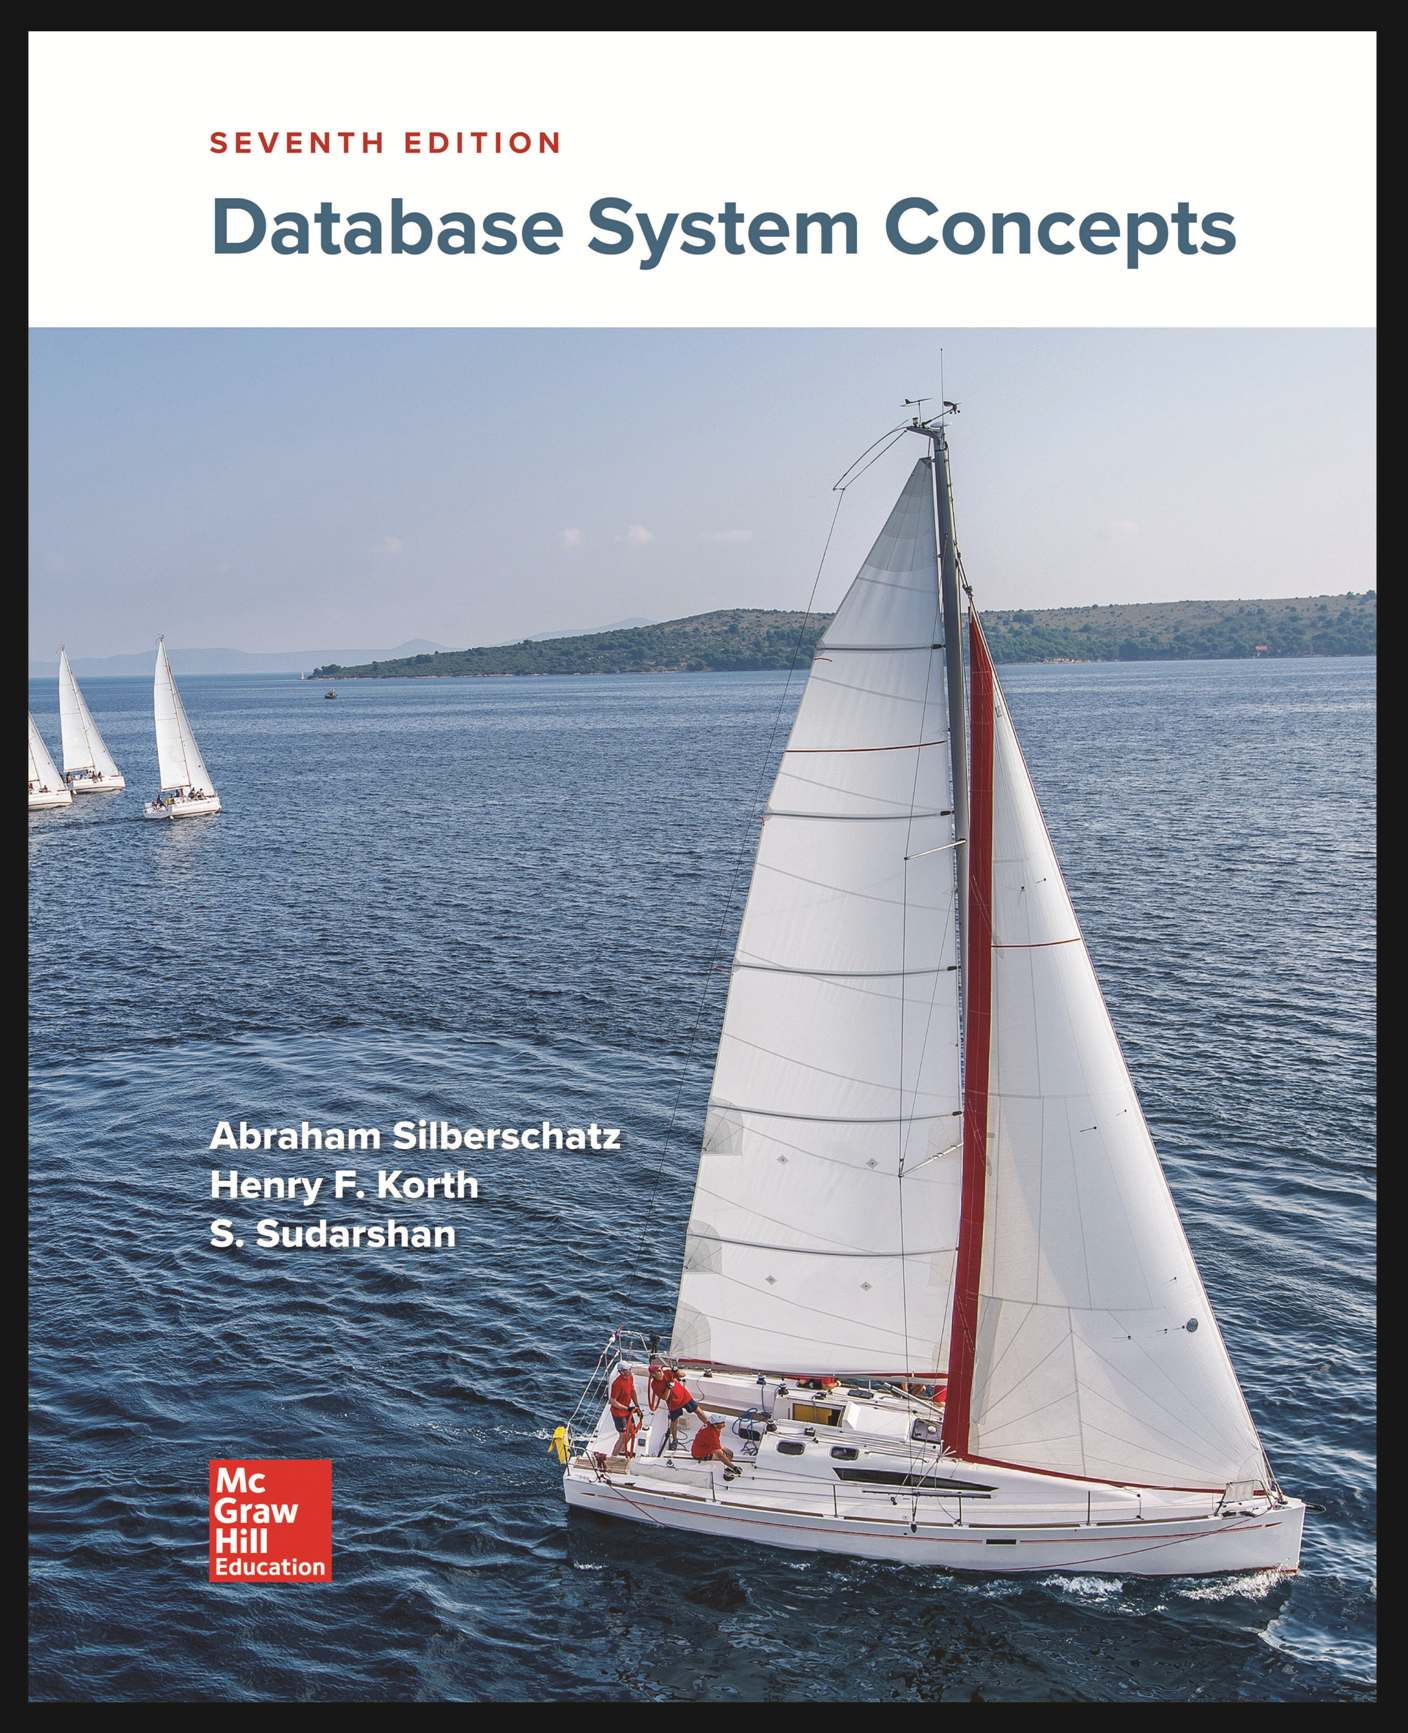
\includegraphics[width=0.5\textwidth]{figures/book_cover.jpg} \\
    \vspace{5mm}
    {
        \tiny
        Content has been extracted from \textit{Database System Concepts}, Seventh Edition, by Silberschatz, Korth and Sudarshan. Mc Graw Hill Education. 2019.\\
        Visit \url{https://db-book.com/}.\\
    }
\end{frame}

\section{Join Expressions}

\begin{frame}{Joined Relations}
    \begin{itemize}
        \item Join operations take two relations and return as a result another relation.
        \item A join operation is a Cartesian product which requires that tuples in the two relations match (under some condition). It also specifies the attributes that are present in the result of the join.
        \item The join operations are typically used as subquery expressions in the \texttt{FROM} clause.
        \item Three types of joins:
        \begin{itemize}
            \item Natural join
            \item Inner join
            \item Outer join
        \end{itemize}
    \end{itemize}
\end{frame}

\begin{frame}[fragile]{Natural Join in SQL}
    \begin{itemize}
        \item Natural join matches tuples with the same values for all common attributes, and retains only one copy of each common column.
        \item For all students in the university who have taken some course, find their names and the course ID of all courses they took.
        \begin{minted}
        [tabsize=4, obeytabs, frame=lines, framesep=2mm, baselinestretch=1.2, bgcolor=LightGray, fontsize=\footnotesize, linenos]{sql}
        SELECT
            name, course_id
        FROM
            students, takes
        WHERE
            student.ID = takes.ID;
        \end{minted}
    \end{itemize}
\end{frame}

\begin{frame}[fragile]{Natural Join in SQL}
    \begin{itemize}
        \item Same query in SQL with ``natural join'' construct.
        \begin{minted}
        [tabsize=4, obeytabs, frame=lines, framesep=2mm, baselinestretch=1.2, bgcolor=LightGray, fontsize=\footnotesize, linenos]{sql}
SELECT
    name, course_id
FROM
    student NATURAL JOIN takes;
        \end{minted}
    \end{itemize}
\end{frame}

\begin{frame}[fragile]{Natural Join in SQL (Cont.)}
    \begin{itemize}
        \item The \texttt{FROM} clause can have multiple relations combined using natural join:
        \begin{lstlisting}[language=SQL]
SELECT @($A_1, A_2, \ldots, A_n$)@
FROM @($r_1$)@ 
    NATURAL JOIN @($r_2$)@ 
    NATURAL JOIN @($\ldots$)@ 
    NATURAL JOIN @($r_n$)@
WHERE @($P$)@;
        \end{lstlisting}
    \end{itemize}
\end{frame}

\begin{frame}{Student Relation}
    \centering
    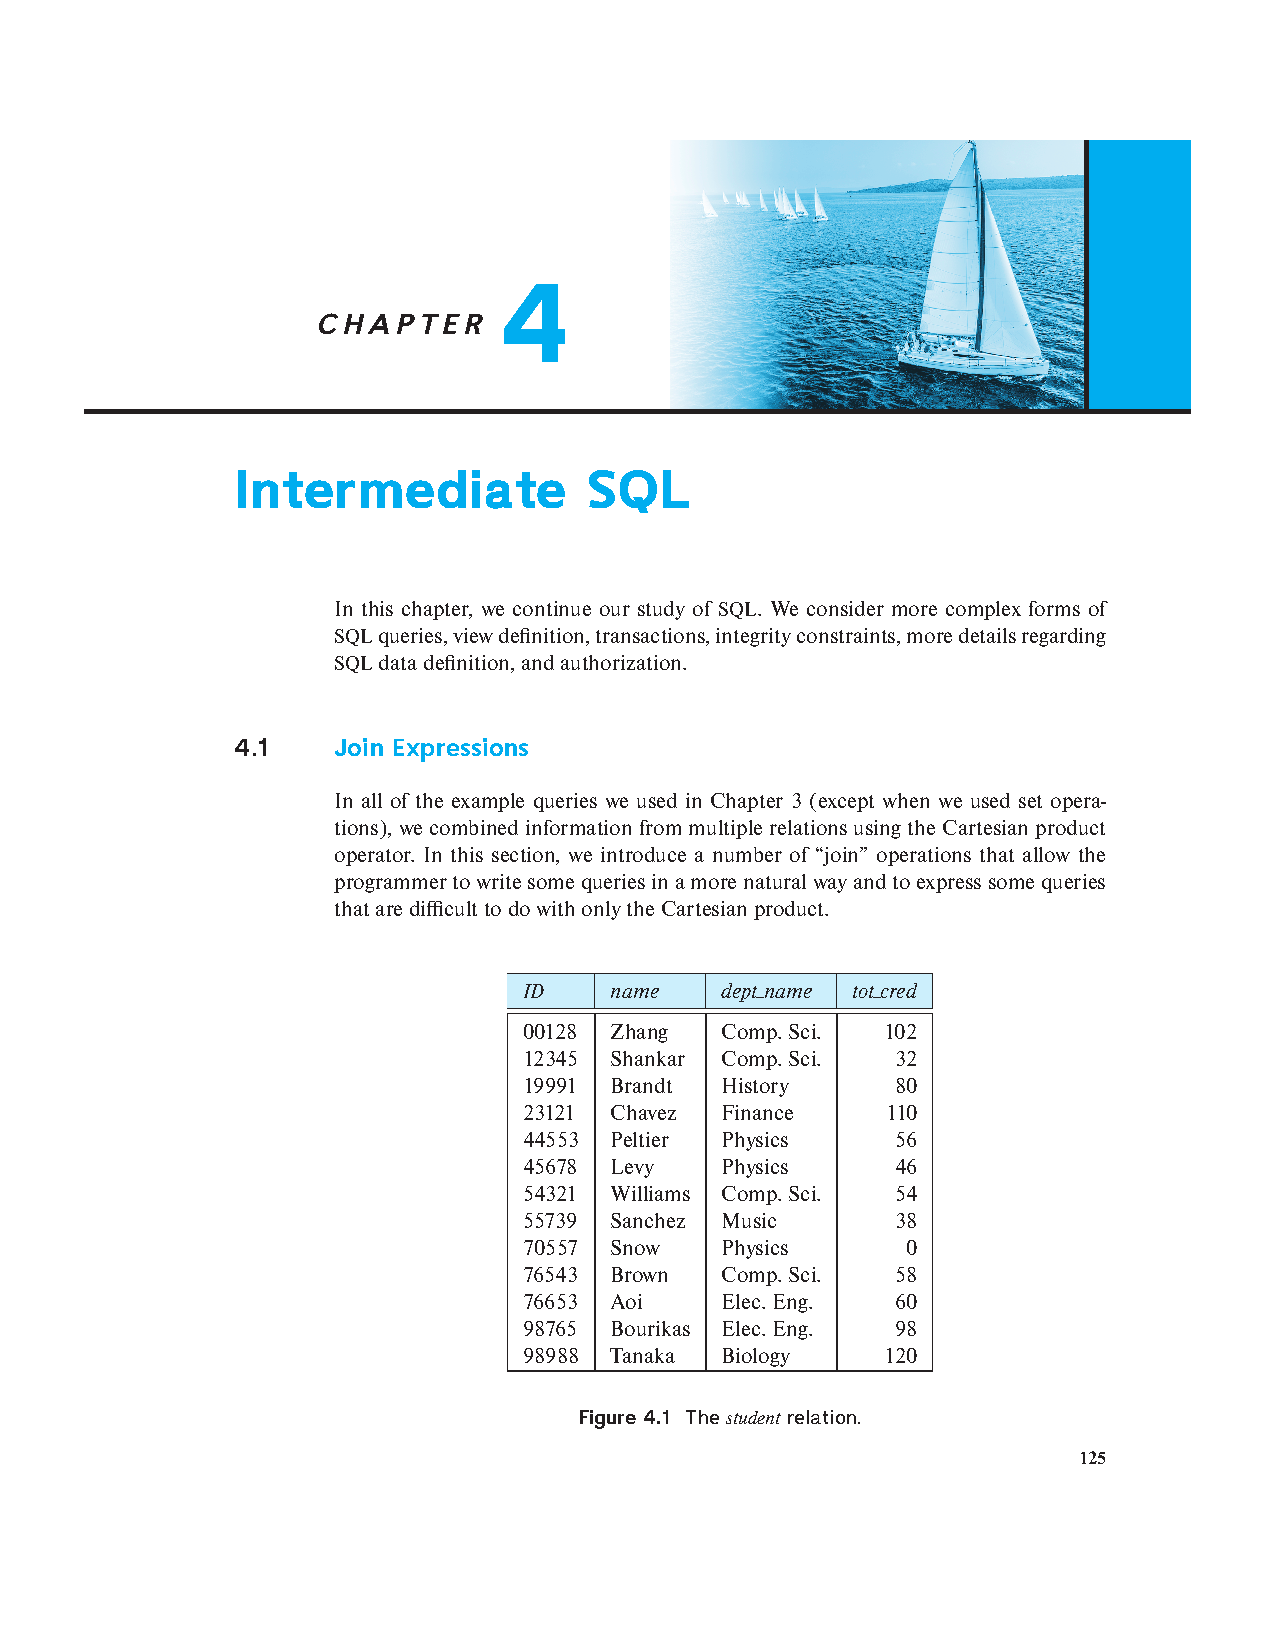
\includegraphics[width=0.75\textwidth, trim={8cm 4.5cm 5cm 16cm}, clip]{pages/nj1.pdf}
\end{frame}

\begin{frame}{Takes Relation}
    \centering
    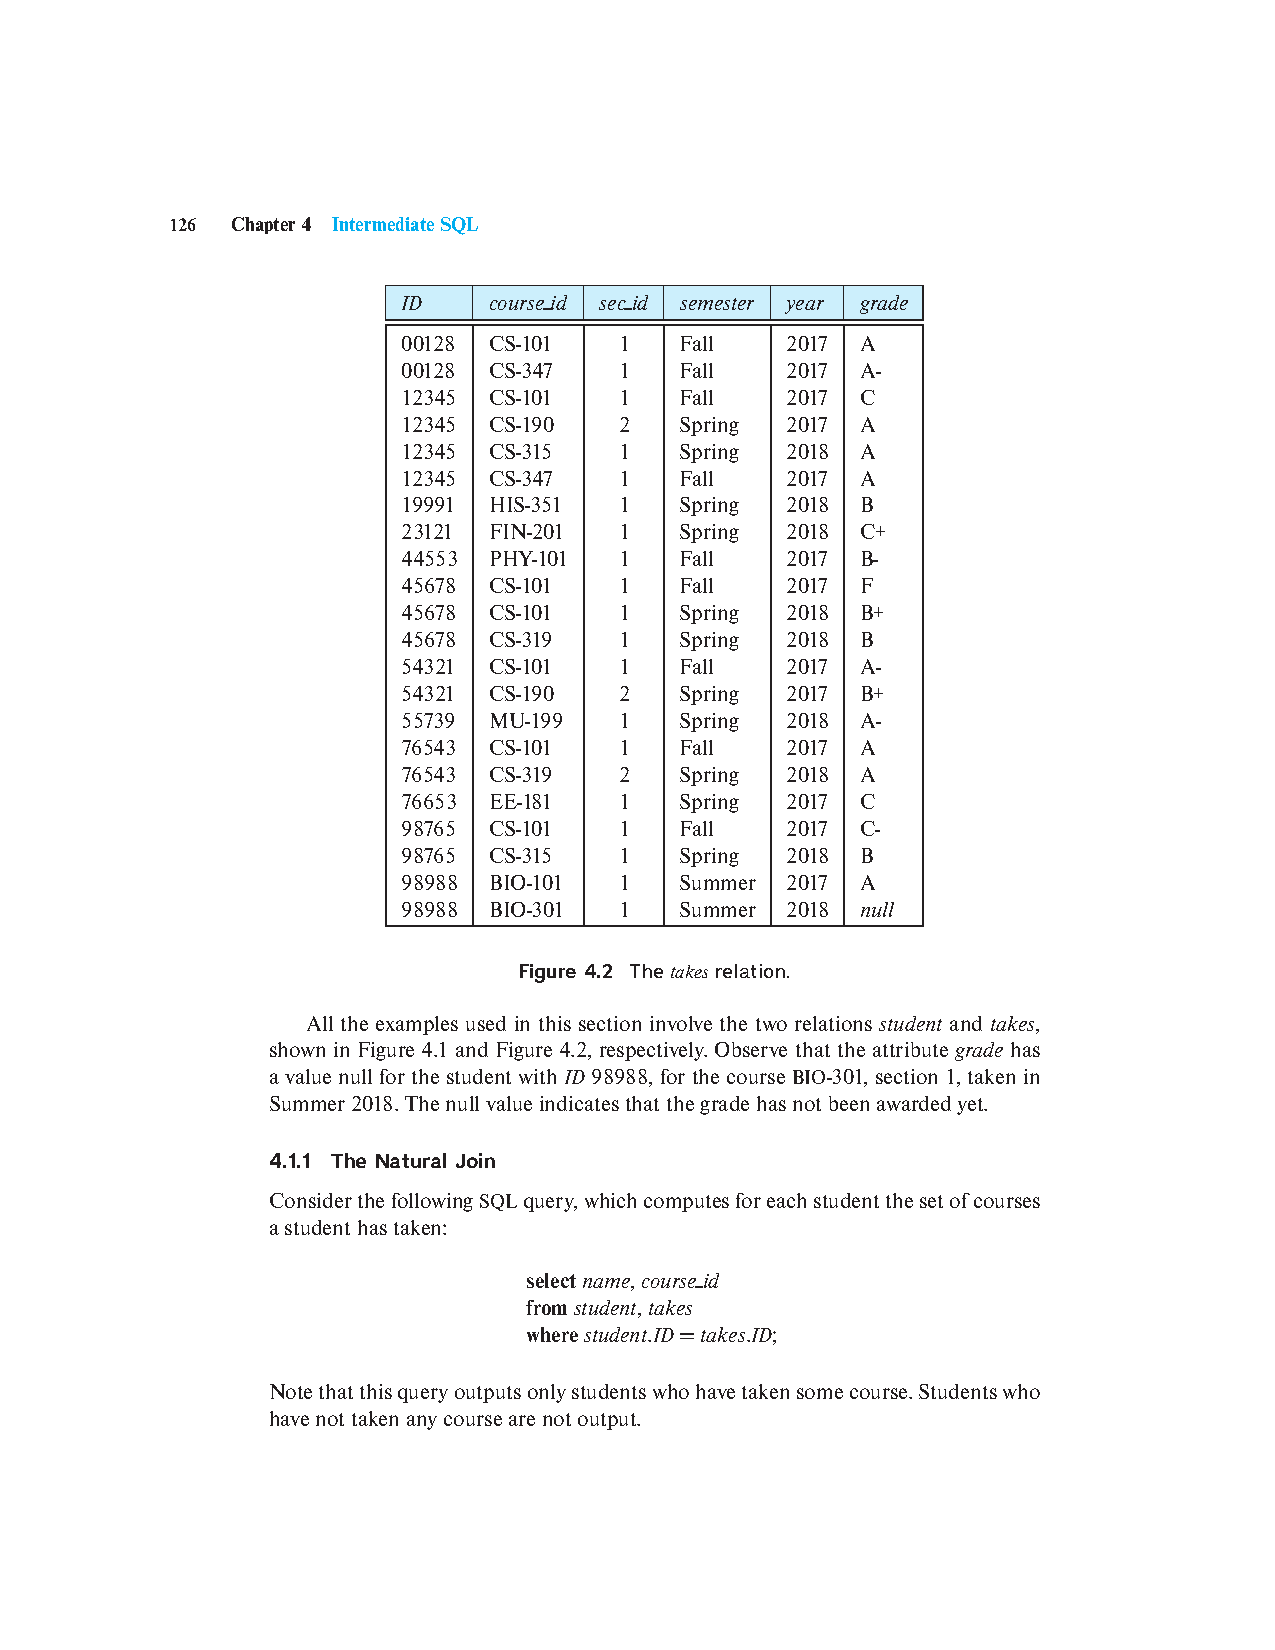
\includegraphics[width=0.75\textwidth, trim={4.5cm 12cm 5.5cm 4.5cm}, clip]{pages/nj2.pdf}
\end{frame}

\begin{frame}{Student Natural Join Takes}
    \centering
    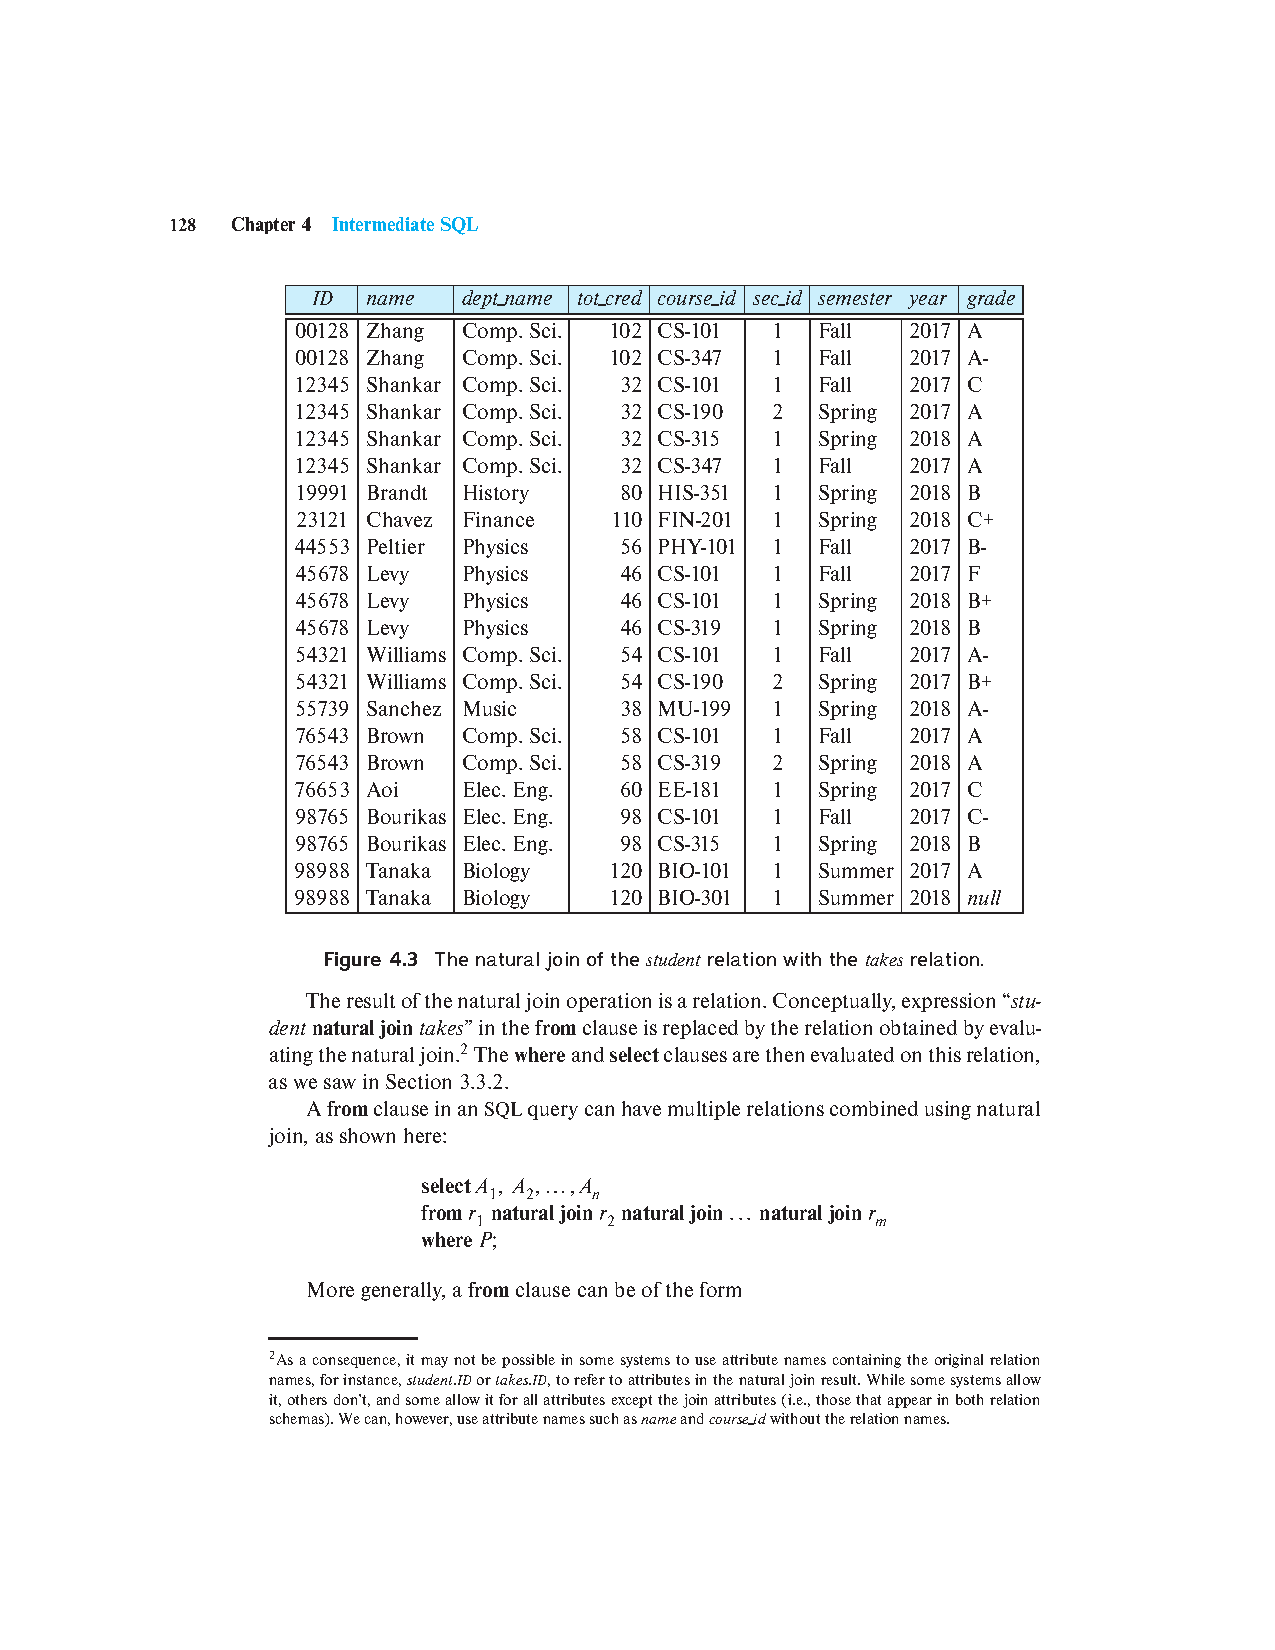
\includegraphics[width=0.95\textwidth, trim={3cm 12cm 3cm 4.5cm}, clip]{pages/nj3.pdf}
\end{frame}

\begin{frame}[fragile]{Dangerous in Natural Join}
    Beware of unrelated attributes with same name which get equated incorrectly
    \begin{exampleblock}{Example:}
        List the names of students along with the titles of courses that they have taken.
    \end{exampleblock}
    \begin{minted}
    [tabsize=4, obeytabs, frame=lines, framesep=2mm, baselinestretch=1.2, bgcolor=LightGray, fontsize=\footnotesize, linenos]{sql}
    SELECT
        name, title
    FROM
        student
    natural join
        takes
    natural join
        course;
    \end{minted}
    \pause
    \vspace{-5mm}
    \begin{FlushRight}
        \Large \textcolor{red}{\textbf{Incorrect!} {\footnotesize double check $dept\_name$ attribute}}
    \end{FlushRight}
\end{frame}

\begin{frame}[fragile]{Dangerous in Natural Join}
    \begin{exampleblock}{Example:}
        List the names of students along with the titles of courses that they have taken.
    \end{exampleblock}
    \begin{minted}
    [tabsize=4, obeytabs, frame=lines, framesep=2mm, baselinestretch=1.2, bgcolor=LightGray, fontsize=\scriptsize, linenos]{sql}
    SELECT
        name, title
    FROM
        student
    NATURAL JOIN
        takes
    NATURAL JOIN
        course;
    \end{minted}
    \begin{itemize}
        \item This query omits all (student name, course title) pairs where the student takes a course in a department other than the student's own department.
    \end{itemize}
\end{frame}

\begin{frame}[fragile]{Dangerous in Natural Join}
    \begin{exampleblock}{Example:}
        List the names of students along with the titles of courses that they have taken.
    \end{exampleblock}
    \begin{minted}
    [tabsize=4, obeytabs, frame=lines, framesep=2mm, baselinestretch=1.2, bgcolor=LightGray, fontsize=\scriptsize, linenos]{sql}
    SELECT
        name, title
    FROM
        student
    NATURAL JOIN
        takes, course
    WHERE
        takes.course_id = course.course_id;
    \end{minted}
    \begin{itemize}
        \item The correct version (above), correctly outputs such pairs.
    \end{itemize}
\end{frame}

\begin{frame}{Outer Join}
    \begin{itemize}
        \item An extension of the join operation that avoids loss of information.
        \item Computes the \texttt{JOIN} and then adds tuples form one relation that does not match tuples in the other relation to the result of the join.
        \item Uses \textbf{\texttt{null}} values.
        \item Three forms of outer join:
        \begin{itemize}
            \item left outer join
            \item right outer join
            \item full outer join
        \end{itemize}
    \end{itemize}
\end{frame}

\begin{frame}{Outer Join Examples}
    \begin{itemize}
        \item Relation \textit{course}: \\
            \vspace{2mm}
            \begin{tabular}{| l | l | l | c |}
                \hline
                \textbf{course\_id} & \textbf{title} & \textbf{dept\_name} & \textbf{credits} \\
                \hline
                BIO-301 & Genetics    & Biology    & 4 \\
                \hline
                CS-190  & Game Design & Comp. Sci. & 4 \\
                \hline
                CS-315  & Robotics    & Comp. Sci. & 3 \\
                \hline
            \end{tabular}
        \item Relation \textit{prereq}: \\
            \vspace{2mm}
            \begin{tabular}{| l | l |}
                \hline
                \textbf{course\_id} & \textbf{prereq\_id} \\
                \hline
                BIO-301 & BIO-101 \\
                \hline
                CS-190  & CS-101  \\
                \hline
                CS-347  & CS-101  \\
                \hline
            \end{tabular}
            \vspace{1mm}
        \item Observe that
        \begin{itemize}
            \item course information is missing for CS-347
            \item prereq information is missing for CS-315
        \end{itemize}
    \end{itemize}
\end{frame}

\begin{frame}{Left Outer Join}
    \begin{itemize}
        \item course \texttt{NATURAL LEFT OUTER JOIN} prereq
    \end{itemize}
    \vspace{5mm}
    \begin{tabular}{| l | l | l | c | l |}
        \hline
        \textbf{course\_id} & \textbf{title} & \textbf{dept\_name} & \textbf{credits} & \textbf{prereq\_id} \\
        \hline
        BIO-301 & Genetics    & Biology    & 4 & BIO-101 \\
        \hline
        CS-190  & Game Design & Comp. Sci. & 4 & CS-101  \\
        \hline
        CS-315  & Robotics    & Comp. Sci. & 3 & \textbf{\texttt{null}}\\
        \hline
    \end{tabular}
    \vspace{5mm}
    \begin{itemize}
        \item In relational algebra: course $\leftouterjoin$ prereq
    \end{itemize}
\end{frame}

\begin{frame}{Right Outer Join}
    \begin{itemize}
        \item course \texttt{NATURAL RIGHT OUTER JOIN} prereq
    \end{itemize}
    \vspace{5mm}
    \begin{tabular}{| l | l | l | c | l |}
        \hline
        \textbf{course\_id} & \textbf{title} & \textbf{dept\_name} & \textbf{credits} & \textbf{prereq\_id} \\
        \hline
        BIO-301 & Genetics    & Biology    & 4 & BIO-101 \\
        \hline
        CS-190  & Game Design & Comp. Sci. & 4 & CS-101  \\
        \hline
        CS-347  & \textbf{\texttt{null}}   & \textbf{\texttt{null}} & \textbf{\texttt{null}} & CS-101 \\
        \hline
    \end{tabular}
    \vspace{5mm}
    \begin{itemize}
        \item In relational algebra: course $\rightouterjoin$ prereq
    \end{itemize}
\end{frame}

\begin{frame}{Full Outer Join}
    \begin{itemize}
        \item course \texttt{NATURAL FULL OUTER JOIN} prereq
    \end{itemize}
    \vspace{5mm}
    \begin{tabular}{| l | l | l | c | l |}
        \hline
        \textbf{course\_id} & \textbf{title} & \textbf{dept\_name} & \textbf{credits} & \textbf{prereq\_id} \\
        \hline
        BIO-301 & Genetics    & Biology    & 4 & BIO-101 \\
        \hline
        CS-190  & Game Design & Comp. Sci. & 4 & CS-101  \\
        \hline
        CS-315  & Robotics    & Comp. Sci. & 3 & \textbf{\texttt{null}}\\
        \hline
        CS-347  & \textbf{\texttt{null}}   & \textbf{\texttt{null}} & \textbf{\texttt{null}} & CS-101 \\
        \hline
    \end{tabular}
    \vspace{5mm}
    \begin{itemize}
        \item In relational algebra: course $\fullouterjoin$ prereq
    \end{itemize}
\end{frame}

\begin{frame}{Joined Types and Conditions}
    \begin{itemize}
        \item \textbf{Join operations} – take two relations and return as a result another relation.
        \item These additional operations are typically used as subquery expressions in the \texttt{FROM} clause
        \item \textbf{Join condition} – defines which tuples in the two relations match, and what attributes are present in the result of the join.
        \item \textbf{Join type} – defines how tuples in each relation that do not match any tuple in the other relation (based on the join condition) are treated.
    \end{itemize}
    \centering
    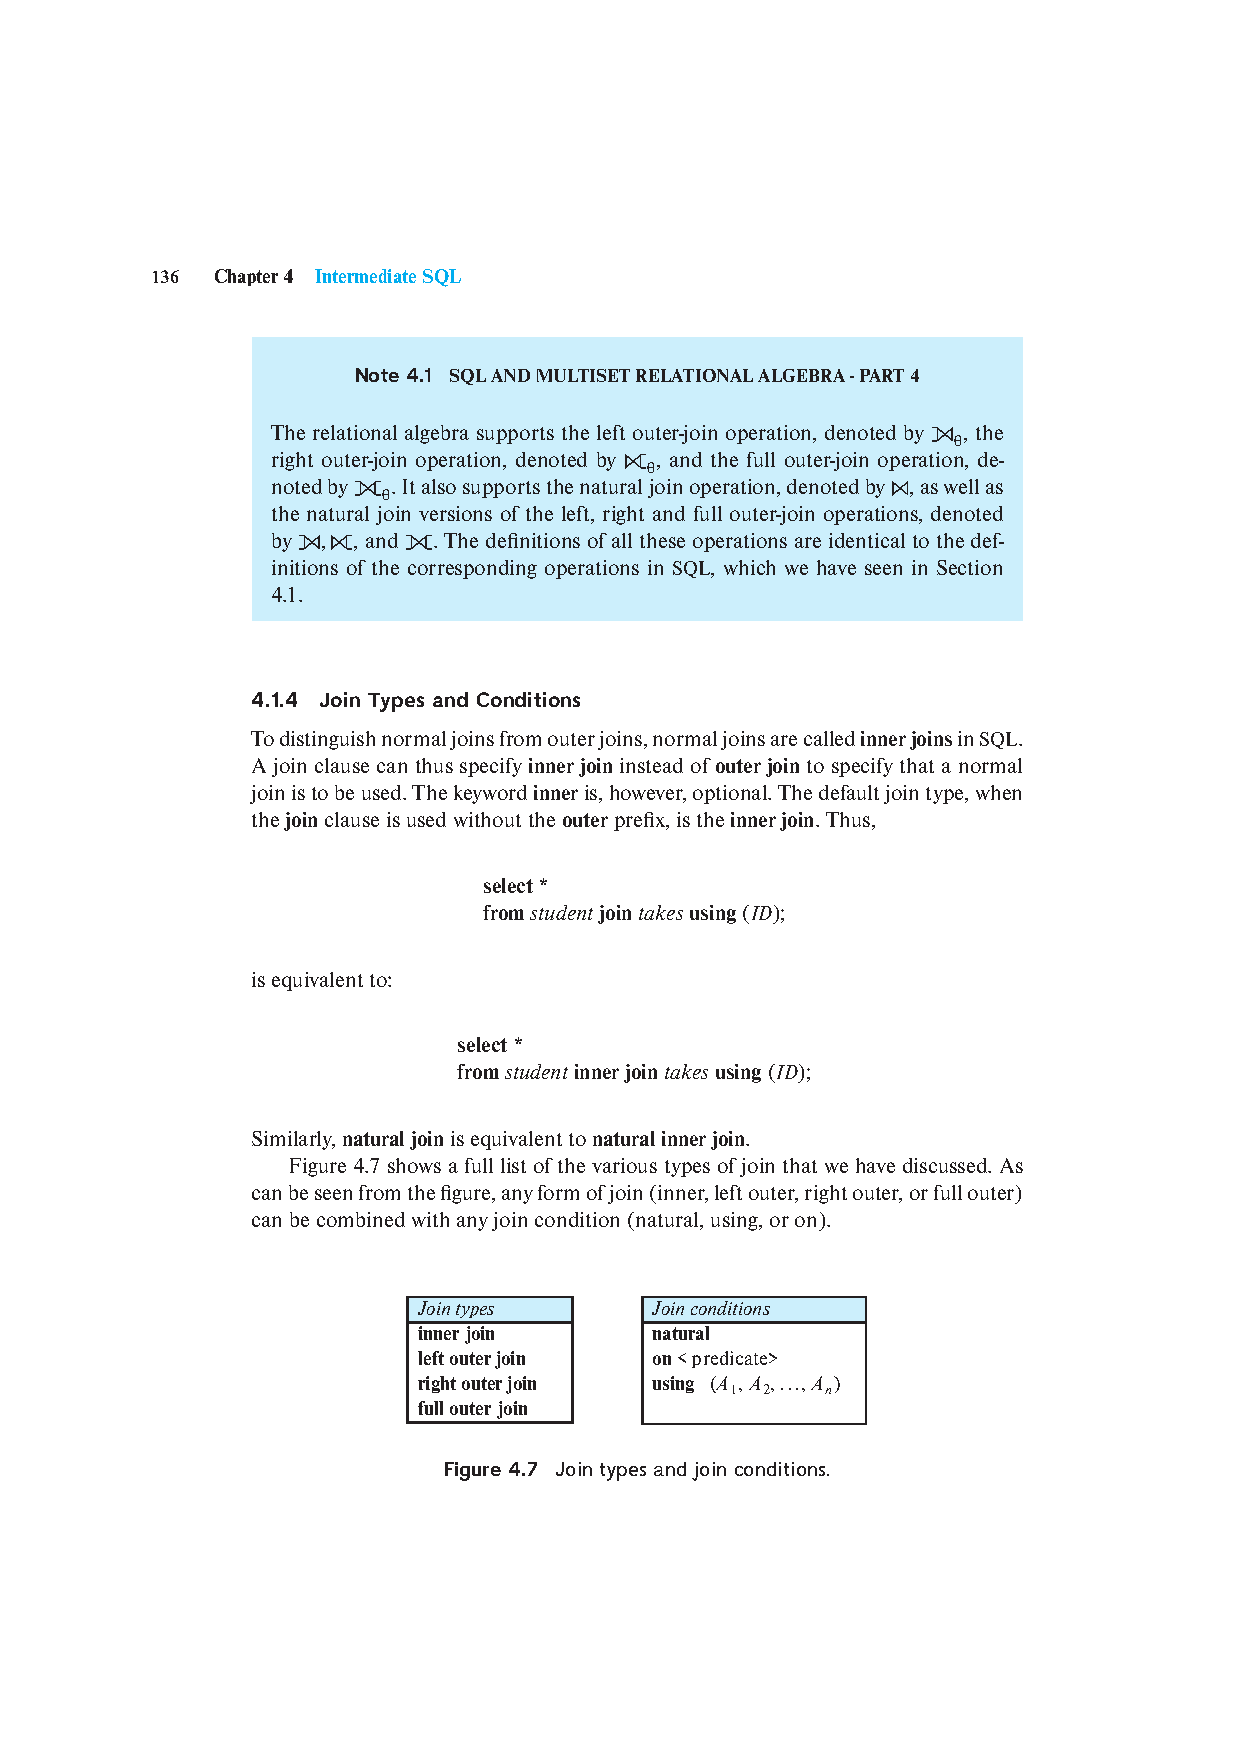
\includegraphics[width=\textwidth, trim={5cm 5.5cm 5cm 21.5cm}, clip]{pages/joins.pdf}
\end{frame}

\begin{frame}{Joined Relations – Examples}
    \begin{itemize}
        \item course \texttt{NATURAL RIGHT OUTER JOIN} prereq
    \end{itemize}
    \scriptsize
    \begin{tabular}{| l | l | l | c | l |}
        \hline
        \textbf{course\_id} & \textbf{title} & \textbf{dept\_name} & \textbf{credits} & \textbf{prereq\_id} \\
        \hline
        BIO-301 & Genetics    & Biology    & 4 & BIO-101 \\
        \hline
        CS-190  & Game Design & Comp. Sci. & 4 & CS-101  \\
        \hline
        CS-347  & \textbf{\texttt{null}}   & \textbf{\texttt{null}} & \textbf{\texttt{null}} & CS-101 \\
        \hline
    \end{tabular}
    \vspace{5mm}
    \normalsize
    \begin{itemize}
        \item course \texttt{FULL OUTER JOIN} prereq \texttt{USING} (course\_id)
    \end{itemize}
    \scriptsize
    \begin{tabular}{| l | l | l | c | l |}
        \hline
        \textbf{course\_id} & \textbf{title} & \textbf{dept\_name} & \textbf{credits} & \textbf{prereq\_id} \\
        \hline
        BIO-301 & Genetics    & Biology    & 4 & BIO-101 \\
        \hline
        CS-190  & Game Design & Comp. Sci. & 4 & CS-101  \\
        \hline
        CS-315  & Robotics    & Comp. Sci. & 3 & \textbf{\texttt{null}}\\
        \hline
        CS-347  & \textbf{\texttt{null}}   & \textbf{\texttt{null}} & \textbf{\texttt{null}} & CS-101 \\
        \hline
    \end{tabular}
\end{frame}

\begin{frame}{Joined Relations – Examples}
    \normalsize
    \begin{itemize}
        \item course \texttt{INNER JOIN} prereq \texttt{ON} course.course\_id = prereq.course\_id
    \end{itemize}
    \scriptsize
    \begin{tabular}{| l | l | l | c | l | l |}
        \hline
        \textbf{course\_id} & \textbf{title} & \textbf{dept\_name} & \textbf{credits} & \textbf{prereq\_id} & \textbf{course\_id} \\
        \hline
        BIO-301 & Genetics    & Biology    & 4 & BIO-101 & BIO-301 \\
        \hline
        CS-190  & Game Design & Comp. Sci. & 4 & CS-101  & CS-190  \\
        \hline
    \end{tabular}
    \normalsize
    \begin{itemize}
        \item What is the difference between the above, and a natural join?
        \vspace{2mm}
        \item course \texttt{LEFT OUTER JOIN} prereq \texttt{ON} course.course\_id = prereq.course\_id
    \end{itemize}
    \scriptsize
    \begin{tabular}{| l | l | l | c | l | l |}
        \hline
        \textbf{course\_id} & \textbf{title} & \textbf{dept\_name} & \textbf{credits} & \textbf{prereq\_id} & \textbf{course\_id} \\
        \hline
        BIO-301 & Genetics    & Biology    & 4 & BIO-101 & BIO-301 \\
        \hline
        CS-190  & Game Design & Comp. Sci. & 4 & CS-101 & CS-190  \\
        \hline
        CS-315  & Robotics    & Comp. Sci. & 3 & \textbf{\texttt{null}} & \textbf{\texttt{null}} \\
        \hline
    \end{tabular}
\end{frame}

\begin{frame}{Joined Relations – Examples}
    \normalsize
    \begin{itemize}
        \item course \texttt{NATURAL RIGHT OUTER JOIN} prereq
    \end{itemize}
    \scriptsize
    \begin{tabular}{| l | l | l | c | l |}
        \hline
        \textbf{course\_id} & \textbf{title} & \textbf{dept\_name} & \textbf{credits} & \textbf{prereq\_id} \\
        \hline
        BIO-301 & Genetics    & Biology    & 4 & BIO-101 \\
        \hline
        CS-190  & Game Design & Comp. Sci. & 4 & CS-101  \\
        \hline
        CS-347  & \texttt{\textbf{null}} & \texttt{\textbf{null}} & \texttt{\textbf{null}} & CS-101  \\
        \hline
    \end{tabular}
    \vspace{5mm}
    \normalsize
    \begin{itemize}
        \item course \texttt{FULL OUTER JOIN} prereq \texttt{USING} (course\_id)
    \end{itemize}
    \scriptsize
    \begin{tabular}{| l | l | l | c | l |}
        \hline
        \textbf{course\_id} & \textbf{title} & \textbf{dept\_name} & \textbf{credits} & \textbf{prereq\_id} \\
        \hline
        BIO-301 & Genetics    & Biology    & 4 & BIO-101 \\
        \hline
        CS-190  & Game Design & Comp. Sci. & 4 & CS-101  \\
        \hline
        CS-315  & Robotics    & Comp. Sci. & 3 & \textbf{\texttt{null}} \\
        \hline
        CS-347  & \texttt{\textbf{null}} & \texttt{\textbf{null}} & \texttt{\textbf{null}} & CS-101  \\
        \hline
    \end{tabular}
\end{frame}

\section{Views}

\begin{frame}[fragile]{Views}
    \begin{itemize}
        \item In some cases, it is not desirable for all users to see the entire logical model (that is, all the actual relations stored in the database.)
        \item Consider a person who needs to know an instructors name and department, but not the salary. This person should see a relation described, in \texttt{SQL}, by
        \begin{minted}
        [tabsize=4, obeytabs, frame=lines, framesep=2mm, baselinestretch=1.2, bgcolor=LightGray, fontsize=\scriptsize, linenos]{sql}
    SELECT
        ID, name, dept_name
    FROM
        instructor;
        \end{minted}
        \item A \textcolor{blue}{\textbf{view}} provides a mechanism to hide certain data from the view of certain users.
        \item Any relation that is not of the conceptual model but is made visible to a user as a “virtual relation” is called a \textbf{\textcolor{blue}{view}}.
    \end{itemize}
\end{frame}

\begin{frame}[fragile]{View Definition}
    \begin{itemize}
        \item A view is defined using the create view statement which has the form:
            \begin{lstlisting}[language=SQL]
    CREATE VIEW v AS @($< query\_expression >$)@;
            \end{lstlisting}
            where $<query\_expression>$ is any legal \texttt{SQL} expression. The view name is represented by v.
        \item Once a view is defined, the view name can be used to refer to the virtual relation that the view generates.
        \item View definition is not the same as creating a new relation by evaluating the query expression
            \begin{itemize}
                \item Rather, a view definition causes the saving of an expression; the expression is substituted into queries using the view.
            \end{itemize}
    \end{itemize}
\end{frame}

\begin{frame}[fragile]{View Definition and Use}
    \begin{itemize}
        \item A view of instructors without their salary.
    \end{itemize}
    \begin{minted}
    [tabsize=4, obeytabs, frame=lines, framesep=2mm, baselinestretch=1.2, bgcolor=LightGray, fontsize=\scriptsize, linenos]{sql}
    CREATE VIEW faculty AS
    SELECT ID, name, dept_name
    FROM instructor
    \end{minted}
    \pause
    \begin{itemize}
        \item Find all instructors in the Biology department
    \end{itemize}
    \begin{minted}
    [tabsize=4, obeytabs, frame=lines, framesep=2mm, baselinestretch=1.2, bgcolor=LightGray, fontsize=\scriptsize, linenos]{sql}
    SELECT name
    FROM faculty
    WHERE dept_name = 'Biology'
    \end{minted}
    \pause
    \begin{itemize}
        \item Create a view of department salary totals
    \end{itemize}
    \begin{minted}
    [tabsize=4, obeytabs, frame=lines, framesep=2mm, baselinestretch=1.2, bgcolor=LightGray, fontsize=\scriptsize, linenos]{sql}
    CREATE VIEW departments_total_salary(dept_name, total_salary) AS
    SELECT dept_name, SUM(salary)
    FROM instructor
    GROUP BY dept_name;
    \end{minted}
\end{frame}

\begin{frame}{Views Defined Using Other Views}
    \begin{itemize}
        \item One view may be used in the expression defining another view.
        \item A view relation $v_1$ is said to \textcolor{blue}{depend directly} on a view relation $v_2$ if $v_2$ is used in the expression defining $v_1$.
        \item A view relation $v_1$ is said to \textcolor{blue}{depend on} view relation $v_2$ if either $v_1$ depends directly to $v_2$ or there is a path of dependencies from $v_1$ to $v_2$.
        \item A view relation $v$ is said to be \textcolor{blue}{recursive} if it depends on itself.
    \end{itemize}
\end{frame}

\begin{frame}[fragile]{Views Defined Using Other Views}
    \begin{minted}
    [tabsize=4, obeytabs, frame=lines, framesep=2mm, baselinestretch=1.2, bgcolor=LightGray, fontsize=\footnotesize, linenos]{sql}
    CREATE VIEW
        physics_fall_2017 AS
    SELECT
        course.course_id, sec_id, building, room_number
    FROM
        course, section
    WHERE
        course.course_id = section.course_id AND
        course.dept_name = 'Physics' AND
        section.semester = 'Fall' AND
        section.year = '2017';
    \end{minted}
\end{frame}

\begin{frame}[fragile]{Views Defined Using Other Views}
    \begin{minted}
    [tabsize=4, obeytabs, frame=lines, framesep=2mm, baselinestretch=1.2, bgcolor=LightGray, fontsize=\footnotesize, linenos]{sql}
    CREATE VIEW
        physics_fall_2017_watson AS
    SELECT
        course_id, room_number
    FROM
        physics_fall_2017
    WHERE
        building= 'Watson';
    \end{minted}
\end{frame}

\begin{frame}[fragile]{View Expansion}
    \begin{itemize}
        \item Expand the view:
            \begin{minted}
            [tabsize=4, obeytabs, frame=lines, framesep=2mm, baselinestretch=1.2, bgcolor=LightGray, fontsize=\scriptsize, linenos]{sql}
CREATE VIEW physics_fall_2017_watson AS
    SELECT course_id, room_number
    FROM physics_fall_2017
    WHERE building= 'Watson';
            \end{minted}
        \item To:
            \begin{minted}
            [tabsize=4, obeytabs, frame=lines, framesep=2mm, baselinestretch=1.2, bgcolor=LightGray, fontsize=\scriptsize, linenos]{sql}
CREATE VIEW physics_fall_2017_watson AS
    SELECT course_id, room_number
    FROM ( SELECT course.course_id, sect_id, building, room_number
            FROM course, section
            WHERE course.course_id = section.course_id
            AND course.dept_name = 'Physics'
            AND section.semester = 'Fall'
            AND section.year = '2017' )
    WHERE building= 'Watson';
            \end{minted}
    \end{itemize}
\end{frame}

\begin{frame}[fragile]{View Expansion (Cont.)}
    \begin{itemize}
        \item A way to define the meaning of views defined in terms of other views.
        \item Let view $v_1$ be defined by an expression $e_1$ that may itself contain uses of view relations.
        \item View expansion of an expression repeats the following replacement step:
            \footnotesize
            \begin{lstlisting}[language=bash]
REPEAT
    Find any view relation @($v_i$)@ in @($e_i$)@
    Replace the view relation @($v_i$)@
        by the expression defining @($v_i$)@
UNTIL no more view relations are present in @($e_i$)@
            \end{lstlisting}
            \normalsize
        \item As long as the view definitions are not recursive, this loop will terminate.
    \end{itemize}
\end{frame}

\begin{frame}{Materialized Views}
    \begin{itemize}
        \item Certain database systems allow view relations to be physically stored.
            \begin{itemize}
                \item Physical copy created when the view is defined.
                \item Such views are called \textbf{\textcolor{blue}{Materialized view}}.
            \end{itemize}
        \item If relations used in the query are updated, the materialized view result becomes out of date.
            \begin{itemize}
                \item Need to \textcolor{blue}{\textbf{maintain}} the view, by updating the view whenever the underlying relations are updated.
            \end{itemize}
    \end{itemize}
\end{frame}

\begin{frame}[fragile]{Update of a View}
    \begin{itemize}
        \item Add a new tuple to faculty view which we defined earlier.
            \begin{minted}
            [tabsize=4, obeytabs, frame=lines, framesep=2mm, baselinestretch=1.2, bgcolor=LightGray, fontsize=\scriptsize]{sql}
    INSERT INTO faculty
    VALUES ('30765', 'Green', 'Music');
            \end{minted}
        \item This insertion must be represented by the insertion into the instructor relation.
            \begin{itemize}
                \item Must have a value for salary.
            \end{itemize}
        \item Two approaches:
            \begin{itemize}
                \item Reject the insert.
                \item Insert the tuple:\\
                    \texttt{(`30765', `Green', `Music', \textbf{null})}\\
                    into the \textit{instructor} relation.
            \end{itemize}
    \end{itemize}
\end{frame}

\begin{frame}[fragile]{Some Updates Cannot be Translated Uniquely}
    \begin{itemize}
        \item[ ]
        \begin{minted}
        [tabsize=4, obeytabs, frame=lines, framesep=2mm, baselinestretch=1.2, bgcolor=LightGray, fontsize=\scriptsize]{sql}
CREATE VIEW instructor_info AS
    SELECT
        ID, name, building
    FROM
        instructor, department
    WHERE
        instructor.dept_name= department.dept_name;
        \end{minted}
        \item[ ]
        \begin{minted}
        [tabsize=4, obeytabs, frame=lines, framesep=2mm, baselinestretch=1.2, bgcolor=LightGray, fontsize=\scriptsize]{sql}
INSERT INTO instructor_info
VALUES ('69987', 'White', 'Taylor');
        \end{minted}
        \pause
        \item Issues:
            \begin{itemize}
                \item Which department, if multiple departments in Taylor?
                \item What if no department is in Taylor?
            \end{itemize}
    \end{itemize}
\end{frame}

\begin{frame}[fragile]{And Some Not at All}
    \begin{itemize}
        \item[ ]
        \begin{minted}
        [tabsize=4, obeytabs, frame=lines, framesep=2mm, baselinestretch=1.2, bgcolor=LightGray, fontsize=\scriptsize]{sql}
CREATE VIEW history_instructors AS
    SELECT *
    FROM instructor
    WHERE dept_name= 'History';
        \end{minted}
        \item What happens if we insert:\\
                \texttt{(`25566', `Brown', `Biology', 100000)}\\
                into \textit{history\_instructors}?
    \end{itemize}
\end{frame}

\begin{frame}{View Updates in SQL}
    \begin{itemize}
        \item Most \texttt{SQL} implementations allow updates only on simple views:
        \begin{itemize}
            \item The \texttt{FROM} clause has only one database relation.
            \item The \texttt{SELECT} clause contains only attribute names of the relation, and does not have any expressions, aggregates, or distinct specification.
            \item Any attribute not listed in the \texttt{SELECT} clause can be set to \texttt{\textbf{null}}.
            \item The query does not have a \texttt{GROUP BY} or \texttt{HAVING} clause.
        \end{itemize}
    \end{itemize}
\end{frame}

\section{Transactions}

\begin{frame}{Transactions}
    \begin{itemize}
        \item A transaction consists of a sequence of query and/or update statements and is a ``unit'' of work.
        \item The \texttt{SQL} standard specifies that a transaction begins implicitly when an \texttt{SQL} statement is executed.
        \item The transaction must end with one of the following statements:
        \begin{itemize}
            \item Commit work. The updates performed by the transaction become permanent in the database.
            \item Rollback work. All the updates performed by the \texttt{SQL} statements in the transaction are undone.
        \end{itemize}
        \item Atomic transaction:
        \begin{itemize}
            \item Either fully executed or rolled back as if it never occurred.
        \end{itemize}
        \item Isolation from concurrent transactions.
    \end{itemize}
\end{frame}

\section{Integrity Constraints}

\begin{frame}{Integrity Constraints}
    \begin{itemize}
        \item Integrity constraints guard against accidental damage to the database, by ensuring that authorized changes to the database do not result in a loss of data consistency.
        \begin{itemize}
            \item A checking account must have a balance greater than \$10,000.00.
            \item A salary of a bank employee must be at least \$4.00 an hour.
            \item A customer must have a (non-null) phone number.
        \end{itemize}
    \end{itemize}
\end{frame}

\begin{frame}{Constraints on a Single Relation}
    \begin{itemize}
        \item not null.
        \item primary key.
        \item unique.
        \item check (P), where P is a predicate.
    \end{itemize}
\end{frame}

\begin{frame}[fragile]{Not Null Constraints}
    \begin{itemize}
        \item \texttt{not null}
        \begin{itemize}
            \item Declare name and budget to be not null:
            \begin{verbatim}
name varchar(20) not null
budget numeric(12,2) not null
            \end{verbatim}
        \end{itemize}
    \end{itemize}
\end{frame}

\begin{frame}[fragile]{Unique Constraints}
    \begin{itemize}
        \item \verb|unique (|$A_1$, $A_2$, $\ldots$, $A_m$ \verb|)|
        \begin{itemize}
            \item The \texttt{unique} specification states that the attributes $A_1, A_2, \ldots, A_m$ form a candidate key.
            \item Candidate keys are permitted to be null (in contrast to primary keys).
        \end{itemize}
    \end{itemize}
\end{frame}

\begin{frame}[fragile]{The check clause}
    \begin{itemize}
        \item The \texttt{check(P)} clause specifies a predicate \texttt{P} that must be satisfied by every tuple in a relation.
        \item Example: Ensure that semester is one of Fall, Winter, Spring or Summer:
    \end{itemize}
    \begin{minted}
    [tabsize=4, obeytabs, frame=lines, framesep=2mm, baselinestretch=1.2, bgcolor=LightGray, fontsize=\footnotesize, linenos]{sql}
CREATE TABLE section (
    course_id varchar (8),
    sec_id varchar (8),
    semester varchar (6),
    year numeric (4,0),
    building varchar (15),
    room_number varchar (7),
    time_slot_id varchar (4),
    PRIMARY KEY (course_id, sec_id, semester, year),
    CHECK(semester in ('Fall', 'Winter', 'Spring', 'Summer'))
);
    \end{minted}
\end{frame}

\begin{frame}{Referential Integrity}
    \begin{itemize}
        \item Ensures that a value that appears in one relation for a given set of attributes also appears for a certain set of attributes in another relation.
        \begin{itemize}
            \item Example: If ``Biology'' is a department name appearing in one of the tuples in the \textit{instructor} relation, then there exists a tuple in the \textit{department} relation for ``Biology''.
        \end{itemize}
        Let $A$ be a set of attributes. Let \texttt{R} and \texttt{S} be two relations that contain attributes $A$ and where $A$ is the primary key of \texttt{S}.  $A$ is said to be a foreign key of \texttt{R} if for any values of $A$ appearing in \texttt{R} these values also appear in \texttt{S}.
    \end{itemize}
\end{frame}

\begin{frame}[fragile]{Referential Integrity (Cont.)}
    \begin{itemize}
        \item Foreign keys can be specified as part of the \texttt{CREATE TABLE} statement:
            \begin{verbatim}
FOREIGN KEY (dept_name) REFERENCES department 
            \end{verbatim}
        \item By default, a foreign key references the primary key attributes of the referenced table.
        \item \texttt{SQL} allows a list of attributes of the referenced relation to be specified explicitly:
            \begin{verbatim}
FOREIGN KEY (dept_name) 
REFERENCES department (dept_name)
            \end{verbatim}
    \end{itemize}
\end{frame}

\begin{frame}[fragile]{Cascading Actions in Referential Integrity}
    \begin{itemize}
        \item When a referential-integrity constraint is violated, the normal procedure is to reject the action that caused the violation.
        \item An alternative, in case of delete or update is to cascade:
        \begin{minted}
        [tabsize=4, obeytabs, frame=lines, framesep=2mm, baselinestretch=1.2, bgcolor=LightGray, fontsize=\footnotesize, linenos]{sql}
CREATE TABLE course (
    ...
    dept_name varchar(20),
    FOREIGN KEY (dept_name) REFERENCES department
        ON DELETE CASCADE
        ON UPDATE CASCADE,
        ...
);        
        \end{minted}
        \item Instead of \texttt{CASCADE} we can use :
        \begin{itemize}
            \item \texttt{SET NULL}
            \item \texttt{SET DEFAULT}
        \end{itemize}
    \end{itemize}
\end{frame}

\begin{frame}[fragile]{Integrity Constraint Violation During Transactions}
    \begin{itemize}
        \item Consider:
        \begin{minted}
        [tabsize=4, obeytabs, frame=lines, framesep=2mm, baselinestretch=1.2, bgcolor=LightGray, fontsize=\scriptsize, linenos]{sql}
CREATE TABLE person (
    ID char(10),
    name char(40),
    mother char(10),
    father char(10),
    PRIMARY KEY ID,
    FOREIGN KEY father REFERENCES person,
    FOREIGN KEY mother REFERENCES person
);        
        \end{minted}
        \item How to insert a tuple without causing constraint violation? \pause
        \begin{itemize}
            \item Insert father and mother of a person before inserting person,
            \item OR, set father and mother to \texttt{\textbf{null}} initially, update after inserting all persons (not possible if father and mother attributes declared to be \texttt{NOT NULL}),
            \item OR defer constraint checking.
        \end{itemize}
    \end{itemize}
\end{frame}

\begin{frame}[fragile]{Complex Check Conditions}
    \begin{itemize}
        \item The predicate in the \texttt{CHECK} clause can be an arbitrary predicate that can include a subquery:
        \begin{verbatim}
CHECK (
    time_slot_id IN (
        SELECT time_slot_id FROM time_slot
    )
)
        \end{verbatim}
        \vspace{-3mm}
        The \texttt{CHECK} condition states that the \texttt{time\_slot\_id} in each tuple in the \textit{section} relation is actually the identifier of a time slot in the \textit{time\_slot} relation.
        \item The condition has to be checked not only when a tuple is inserted or modified in \textit{section}, but also when the relation \textit{time\_slot} changes.
    \end{itemize}
\end{frame}

\begin{frame}[fragile]{Assertions}
    \begin{itemize}
        \item An assertion is a predicate expressing a condition that we wish the database always to satisfy.
        \item The following constraints, can be expressed using assertions:
        \begin{itemize}
            \item For each tuple in the \textit{student} relation, the value of the attribute \texttt{tot\_cred} must equal the sum of credits of courses that the student has completed successfully.
            \item An instructor cannot teach in two different classrooms in a semester in the same time slot.
        \end{itemize}
        \item An assertion in SQL takes the form:
        \begin{minted}
        [tabsize=4, obeytabs, frame=lines, framesep=2mm, baselinestretch=1.2, bgcolor=LightGray, fontsize=\footnotesize]{sql}
CREATE ASSERTION <assertion-name> CHECK (<predicate>);
        \end{minted}
    \end{itemize}
\end{frame}

\section{SQL Data Types and Schemas}

\begin{frame}[fragile]{Built-in Data Types in SQL}
    \begin{itemize}
        \item \texttt{date}: Dates, containing a (4 digit) year, month and date:
        \begin{itemize}
            \item Example: \verb|date '2005-7-27'|
        \end{itemize}
        \item \texttt{time}: Time of day, in hours, minutes and seconds.
        \begin{itemize}
            \item Example: \verb|time '09:00:30'|,  \verb|time '09:00:30.75'|
        \end{itemize}
        \item \texttt{timestamp}: date plus time of day.
        \begin{itemize}
            \item Example: \verb|timestamp '2005-7-27 09:00:30.75'|
        \end{itemize}
        \item \texttt{interval}: period of time.
        \begin{itemize}
            \item Example: \verb|interval '1' day|
            \item Subtracting a date/time/timestamp value from another gives an interval value.
            \item Interval values can be added to date/time/timestamp values.
        \end{itemize}
    \end{itemize}
\end{frame}

\begin{frame}{Large-Object Types}
    \begin{itemize}
        \item Large objects (photos, videos, CAD files, etc.) are stored as a large object:
        \begin{itemize}
            \item \textbf{blob}: binary large object -- object is a large collection of uninterpreted binary data (whose interpretation is left to an application outside of the database system).
            \item \textbf{clob}: character large object -- object is a large collection of character data.
        \end{itemize}
        \item When a query returns a large object, a pointer is returned rather than the large object itself.
    \end{itemize}
\end{frame}

\begin{frame}[fragile]{User-Defined Types}
    \begin{itemize}
        \item \texttt{CREATE TYPE} construct in \texttt{SQL} creates user-defined type:
        \begin{verbatim}
CREATE TYPE Dollars AS numeric (12,2) final
        \end{verbatim}

        \item Example:
        \begin{minted}
        [tabsize=4, obeytabs, frame=lines, framesep=2mm, baselinestretch=1.2, bgcolor=LightGray, fontsize=\footnotesize, linenos]{sql}
CREATE TABLE department (
    dept_name varchar (20),
    building varchar (15),
    budget Dollars
);
        \end{minted}
    \end{itemize}
\end{frame}

\begin{frame}[fragile]{Domains}
    \begin{itemize}
        \item \texttt{CREATE DOMAIN} construct in SQL-92 creates user-defined domain types:
        \begin{verbatim}         
CREATE DOMAIN person_name char(20) NOT NULL
        \end{verbatim}
        \item Types and domains are similar. Domains can have constraints, such as \texttt{NOT NULL}, specified on them.
        \item Example:
        \begin{minted}
        [tabsize=4, obeytabs, frame=lines, framesep=2mm, baselinestretch=1.2, bgcolor=LightGray, fontsize=\footnotesize, linenos]{sql}
CREATE DOMAIN degree_level varchar(10)
CONSTRAINT degree_level_test
    CHECK(
        degree_value IN 
        ('Bachelors', 'Masters', 'Doctorate')
    );
        \end{minted}
    \end{itemize}
\end{frame}

\section{Index Definition in SQL}

\begin{frame}[fragile]{Index Creation}
    \begin{itemize}
        \item Many queries reference only a small proportion of the records in a table.
        \item It is inefficient for the system to read every record to find a record with particular value
        \item An index on an attribute of a relation is a data structure that allows the database system to find those tuples in the relation that have a specified value for that attribute efficiently, without scanning through all the tuples of the relation.
        \item We create an index with the \texttt{CREATE INDEX} command:
        \begin{verbatim}         
CREATE INDEX <name> ON <relation-name> (attribute);
        \end{verbatim}
    \end{itemize}
\end{frame}

\begin{frame}[fragile]{Index Creation Example}
    \begin{minted}
    [tabsize=4, obeytabs, frame=lines, framesep=2mm, baselinestretch=1.2, bgcolor=LightGray, fontsize=\scriptsize, linenos]{sql}
CREATE TABLE student(
    ID varchar (5),
    name varchar (20) NOT NULL,
    dept_name varchar (20),
    tot_cred numeric (3,0) DEFAULT 0,
    PRIMARY KEY (ID)
);

CREATE INDEX studentID_index ON student(ID);
    \end{minted}
    \footnotesize
    \begin{itemize}
        \item The query:
        \begin{minted}
        [tabsize=4, obeytabs, frame=lines, framesep=2mm, baselinestretch=1.2, bgcolor=LightGray, fontsize=\scriptsize, linenos]{sql}
SELECT *
FROM student
WHERE ID = '12345';
        \end{minted}
        can be executed by using the index to find the required record, without looking at all records of \textit{student}.
    \end{itemize}
\end{frame}

\section{Authorization}

\begin{frame}{Authorization}
    \begin{itemize}
        \item We may assign a user several forms of authorizations on parts of the database.
        \begin{itemize}
            \item \textbf{Read} - allows reading, but not modification of data.
            \item \textbf{Insert} - allows insertion of new data, but not modification of existing data.
            \item \textbf{Update} - allows modification, but not deletion of data.
            \item \textbf{Delete} - allows deletion of data.
        \end{itemize}
        \item Each of these types of authorizations is called a \textbf{privilege}.  We may authorize the user all, none, or a combination of these types of privileges on specified parts of a database, such as a relation or a view.
    \end{itemize}
\end{frame}

\begin{frame}{Authorization (Cont.)}
    \begin{itemize}
        \item Forms of authorization to modify the database schema.
        \begin{itemize}
            \item \textbf{Index} - allows creation and deletion of indices.
            \item \textbf{Resources} - allows creation of new relations.
            \item \textbf{Alteration} - allows addition or deletion of attributes in a relation.
            \item \textbf{Drop} - allows deletion of relations.
        \end{itemize}
    \end{itemize}
\end{frame}

\begin{frame}[fragile]{Authorization Specification in SQL}
    \begin{itemize}
        \item The grant statement is used to confer authorization:
            \begin{verbatim}
GRANT <privilege list> ON <relation or view >
    TO <user list>
            \end{verbatim}
        \item \verb|<user list>|is:
            \begin{itemize}
                \item a user-id.
                \item \textbf{public}, which allows all valid users the privilege granted.
                \item A role (more on this later).
            \end{itemize}
        \item Example:
            \begin{itemize}
                \item
                \begin{verbatim}
GRANT SELECT ON department TO Amit, Satoshi
                \end{verbatim}
            \end{itemize}
        \item Granting a privilege on a view does not imply granting any privileges on the underlying relations.
        \item The grantor of the privilege must already hold the privilege on the specified item (or be the database administrator).
    \end{itemize}
\end{frame}

\begin{frame}[fragile]{Privileges in SQL}
    \begin{itemize}
        \item \texttt{SELECT}: allows read access to relation, or the ability to query using the view.
            \begin{itemize}
                \item Example: grant users $U_1$, $U_2$, and $U_3$ \textbf{select} authorization on the \textit{instructor} relation:
                    \begin{lstlisting}
 GRANT SELECT ON instructor TO @($U_1$)@, @($U_2$)@, @($U_3$)@;
                    \end{lstlisting}
            \end{itemize}
        \item \texttt{INSERT}: the ability to insert tuples.
        \item \texttt{UPDATE}: the ability to update using the SQL update statement.
        \item \texttt{DELETE}: the ability to delete tuples.
        \item \texttt{ALL PRIVILEGES}: used as a short form for all the allowable privileges.
    \end{itemize}
\end{frame}

\begin{frame}[fragile]{Revoking Authorization in SQL}
    \begin{itemize}
        \item The revoke statement is used to revoke authorization.
            \begin{verbatim}
    REVOKE <privilege list>
    ON <relation or view>
    FROM <revokee list>
            \end{verbatim}
        \item Example:
            \begin{lstlisting}
 REVOKE SELECT ON instructor TO @($U_1$)@, @($U_2$)@, @($U_3$)@;
            \end{lstlisting}
        \item \verb|<privilege-list>| may be all to revoke all privileges the revokee may hold.
        \item If \verb|<revokee list>| includes \textbf{public}, all users lose the privilege except those granted it explicitly.
        \item If the same privilege was granted twice to the same user by different grantees, the user may retain the privilege after the revocation.
        \item All privileges that depend on the privilege being revoked are also revoked.
    \end{itemize}
\end{frame}

\begin{frame}[fragile]{Roles}
    \begin{itemize}
        \item A role is a way to distinguish among various users as far as what these users can access/update in the database.
        \item To create a role we use:
            \begin{verbatim}
    CREATE ROLE <name>
            \end{verbatim}
        \item Example:
            \begin{verbatim}
    CREATE ROLE instructor
            \end{verbatim}
        \item Once a role is created we can assign ``users'' to the role using:
            \begin{verbatim}
    GRANT <role> TO <users>
            \end{verbatim}
    \end{itemize}
\end{frame}

\begin{frame}[fragile]{Roles Example}
    \footnotesize
    \begin{itemize}
        \item[ ]
            \begin{minted}
            [tabsize=4, obeytabs, frame=lines, framesep=2mm, baselinestretch=1.2, bgcolor=LightGray, fontsize=\scriptsize]{sql}
CREATE ROLE instructor;
GRANT instructor TO Amit;
            \end{minted}
            \pause
        \item Privileges can be granted to roles:
            \begin{minted}
            [tabsize=4, obeytabs, frame=lines, framesep=2mm, baselinestretch=1.2, bgcolor=LightGray, fontsize=\scriptsize]{sql}
GRANT SELECT ON takes TO instructor;
            \end{minted}
            \pause
        \item Roles can be granted to users, as well as to other roles:
            \begin{itemize}
                \begin{minted}
                [tabsize=4, obeytabs, frame=lines, framesep=2mm, baselinestretch=1.2, bgcolor=LightGray, fontsize=\scriptsize]{sql}
CREATE ROLE teaching_assistant;
GRANT teaching_assistant TO instructor;
                \end{minted}
                \begin{itemize}
                    \item \texttt{instructor} inherits all privileges of \texttt{teaching\_assistant}.
                \end{itemize}
            \end{itemize} \pause
        \item Chain of roles:
            \begin{minted}
            [tabsize=4, obeytabs, frame=lines, framesep=2mm, baselinestretch=1.2, bgcolor=LightGray, fontsize=\scriptsize]{sql}
CREATE ROLE dean;
GRANT instructor TO dean;
GRANT dean TO Satoshi;
            \end{minted}
    \end{itemize}
\end{frame}

\begin{frame}[fragile]{Authorization on Views}
    \begin{itemize}
        \item[ ]
            \begin{minted}
            [tabsize=4, obeytabs, frame=lines, framesep=2mm, baselinestretch=1.2, bgcolor=LightGray, fontsize=\scriptsize, linenos]{sql}
CREATE VIEW geo_instructor AS (
    SELECT *
    FROM instructor
    WHERE dept_name = 'Geology'
);
GRANT SELECT ON geo_instructor TO geo_staff;
            \end{minted}
        \pause
        \item Suppose that a \verb|geo_staff| member issues:
            \begin{minted}
            [tabsize=4, obeytabs, frame=lines, framesep=2mm, baselinestretch=1.2, bgcolor=LightGray, fontsize=\scriptsize]{sql}
SELECT *
FROM geo_instructor;
            \end{minted}
        \pause
        \item What if:
        \begin{itemize}
            \item \verb|geo_staff| does not have permissions on \textit{instructor}?
            \item creator of view did not have some permissions on \textit{instructor}?
        \end{itemize}
    \end{itemize}
\end{frame}

\begin{frame}[fragile]{Other Authorization Features}
    \begin{itemize}
        \item \texttt{REFERENCES} privilege to create foreign key:
            \begin{itemize}
                \item[ ] \text{ }
                    \begin{minted}
                    [tabsize=4, obeytabs, frame=lines, framesep=2mm, baselinestretch=1.2, bgcolor=LightGray, fontsize=\scriptsize]{sql}
GRANT REFERENCE (dept_name) ON department TO Mariano;
                    \end{minted}
                \item Why is this required?
            \end{itemize}
        \item Transfer of privileges:
            \begin{itemize}
                \item[ ] \text{ }
                    \begin{minted}
                    [tabsize=4, obeytabs, frame=lines, framesep=2mm, baselinestretch=1.2, bgcolor=LightGray, fontsize=\scriptsize]{sql}
GRANT SELECT ON department TO Amit WITH GRANT OPTION;
REVOKE SELECT ON department FROM Amit, Satoshi CASCADE;
REVOKE SELECT ON department FROM Amit, Satoshi RESTRICT;
                    \end{minted}
                \item And more!
            \end{itemize}
    \end{itemize}
\end{frame}

\begin{frame}{}
     \centering
     \Huge End of Chapter 4.
\end{frame}

\section*{Takeaways}

% Tim Duncan's Top 5 Fundamental Takeaways of Today's Class
\begin{frame}{TDT5FTOTC}
    \centering
    
\includegraphics[width=0.75\textwidth]{figures/tim.png}
\end{frame}

\begin{frame}{Top 5 Fundamental Takeaways}
    \small
    \begin{enumerate}
        \item[5] \textbf{Join Operations in \texttt{SQL}} – \texttt{SQL} joins (natural, inner, and outer) combine tables based on matching attributes, with outer joins preserving unmatched rows using \texttt{\textbf{null}} values.
        \pause
        \item[4] \textbf{Views and Their Uses} – Views are virtual tables that simplify queries and restrict data access, but they are not physically stored unless materialized.
        \pause
        \item[3] \textbf{Transactions and Atomicity} – Transactions ensure database consistency by executing multiple \texttt{SQL} operations as a unit, requiring either a commit to save changes or a rollback to undo them.
        \pause
        \item[2] \textbf{Integrity Constraints and Referential Integrity} – Constraints like \texttt{NOT NULL}, \texttt{PRIMARY KEY}, and foreign keys enforce data integrity, ensuring valid relationships between tables.
        \pause
        \item[1] \textbf{Indexing for Performance Optimization} – Indexes speed up database queries by enabling efficient lookups, reducing the need for full table scans.
    \end{enumerate}
\end{frame}

\begin{frame}{Database System Concepts}
    \centering
    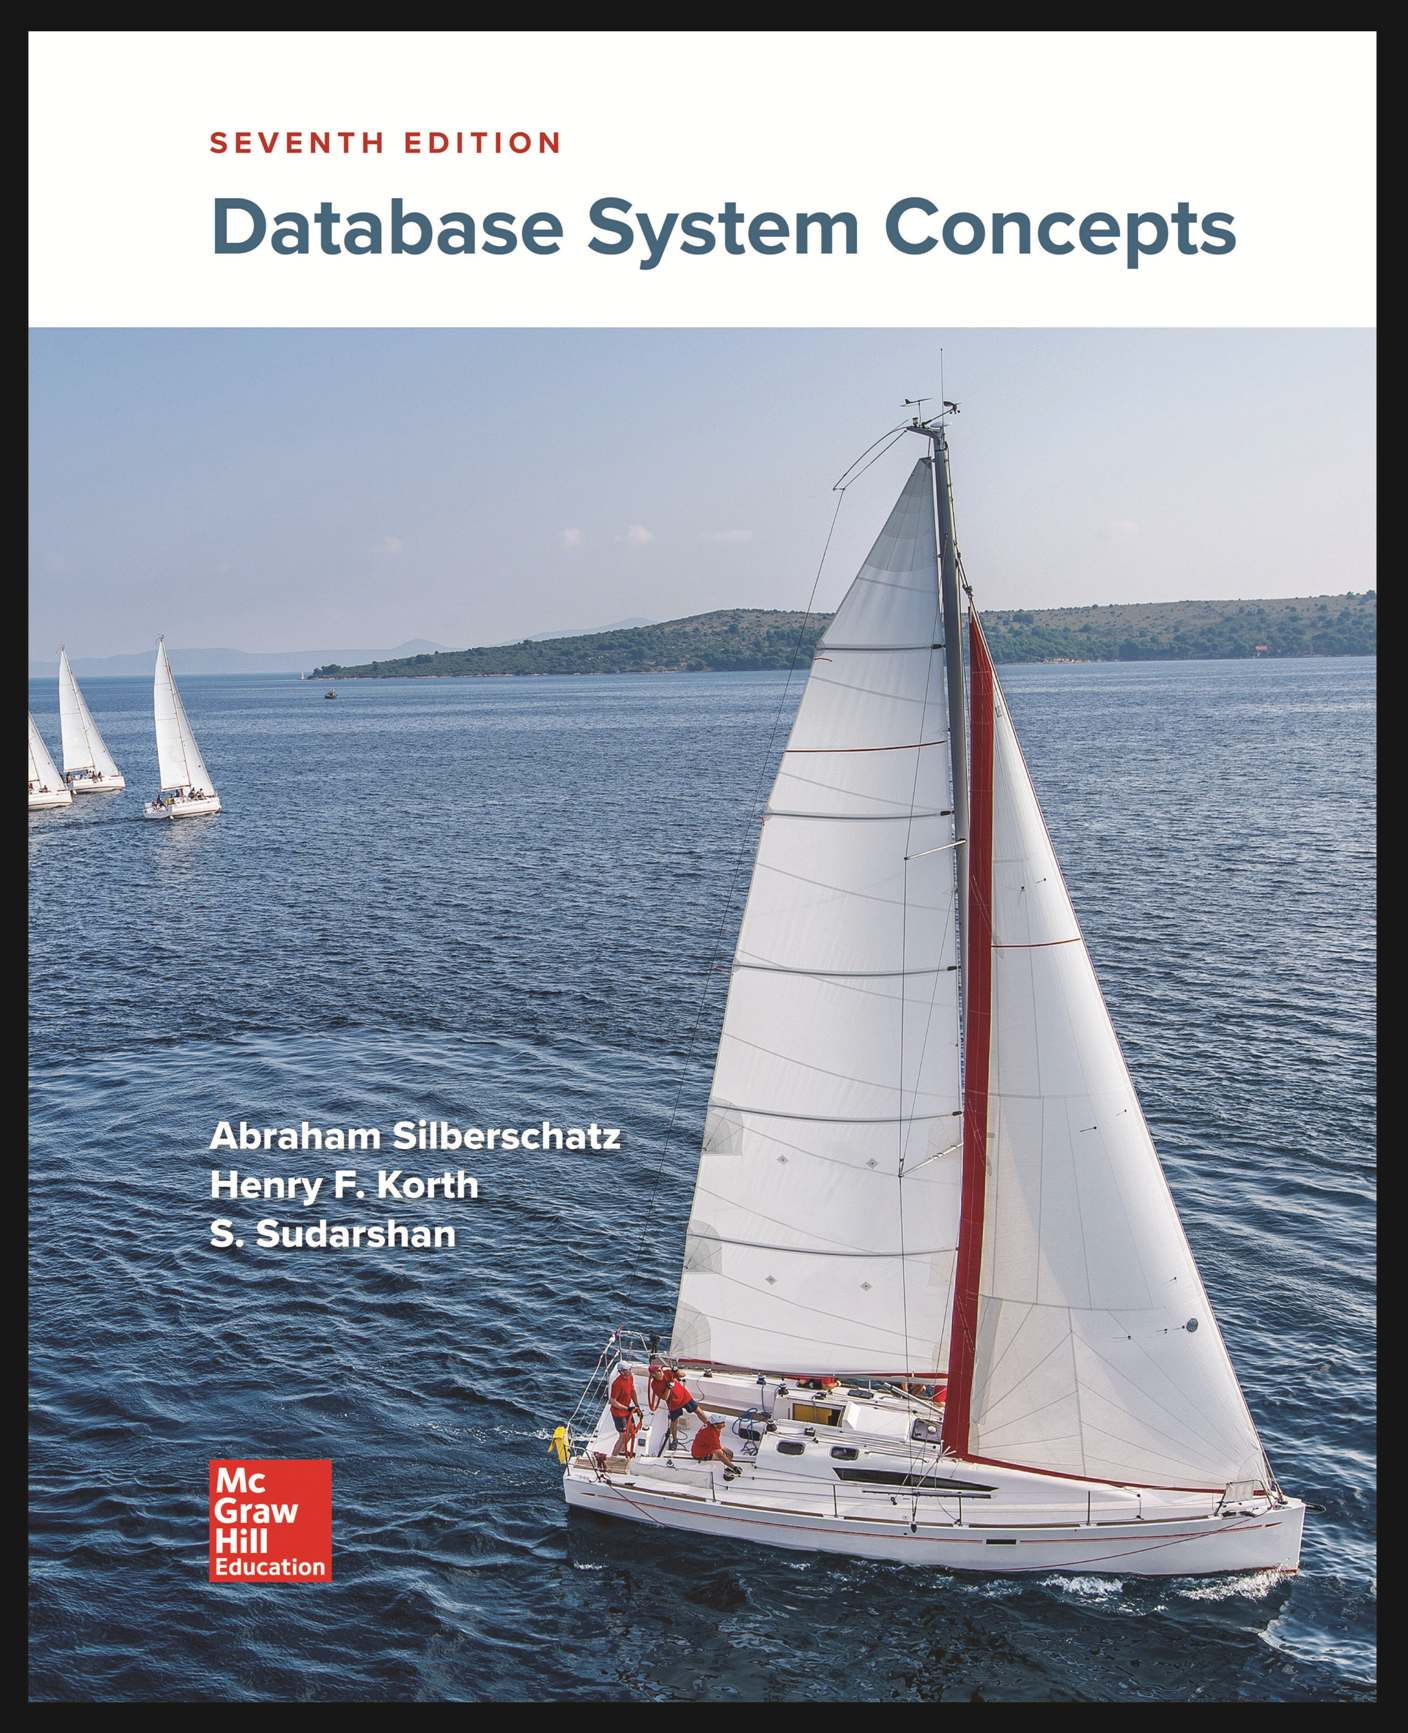
\includegraphics[width=0.5\textwidth]{figures/book_cover.jpg} \\
    \vspace{5mm}
    {
        \tiny
        Content has been extracted from \textit{Database System Concepts}, Seventh Edition, by Silberschatz, Korth and Sudarshan. Mc Graw Hill Education. 2019.\\
        Visit \url{https://db-book.com/}.\\
    }
\end{frame}

\end{document}
